\section{首达时间}
\label{sec:graph-walk-hitting}

前面固定时刻，考察棋子落在何处。现在换一个角度：固定目的地，问棋子在第几步首次到达。每次行走可能走不同的步数。我们先把这个步数当作一个随机量，再计算它的期望。

\subsection{首达期望的方程}
\label{sec:graph-walk-hitting-equation}

在四点路径上从顶点$1$出发，目标是$4$。一种可能是直走三步$1\to2\to3\to4$，另一种可能是走了五步$1\to2\to1\to2\to3\to4$，还有更长的情况。$\tau_4$记录的是某一次试验中实际走出的步数，$h_{1,4}$则是对所有可能步数按概率求出的平均值。

若起点已经是目标，一步也不用走。一般地，对目标$j$定义\term{首达时间}（hitting time）$\tau_j$，并用$h_{i,j}$表示从$i$出发的首达期望，
\begin{equation}
\tau_j=\inf\{t\ge0:X_t=j\},
\qquad h_{i,j}=\mathbb{E}_i[\tau_j].
\label{eq:graph-walk-hitting-definition}
\end{equation}
$\mathbb{E}_i$表示固定$X_0=i$后的期望，且$h_{j,j}=0$。

先检查期望是否有限。对每个非目标顶点选一条通往$j$的简单路径，长度至多$n-1$。沿这些路径逐步走完的最小概率为某个$p>0$。

将行走按每$n-1$步分块。不论上一块结束在什么位置，只要尚未到达目标，下一块命中它的概率至少为$p$。连续$k$块均未命中的概率至多$(1-p)^k$，几何级数求和给出等待的块数期望不超过$1/p$。每块最多$n-1$步，因此$h_{i,j}\le(n-1)/p$。

\paragraph{首步分解}

从$i\ne j$出发，第一步总要花一步。若这一步走到$k$，剩余等待时间的期望正是$h_{k,j}$，因为以后的转移只取决于当前位置。按第一步的去向加权求和，得到
\begin{equation}
h_{i,j}=1+\sum_k P_{i,k}h_{k,j},\qquad i\ne j.
\label{eq:graph-walk-first-step}
\end{equation}

\paragraph{化为拉普拉斯方程}

用$P_{i,k}=w_{i,k}/d_i$代入上式并两边乘$d_i$，一步的代价$1$变成$d_i$，
\[
d_i h_{i,j}-\sum_k w_{i,k}h_{k,j}=d_i,\qquad i\ne j.
\]
左边正是$\bm{D}-\bm{W}=\bm{L}$作用于首达期望列$\bm{h}_{:,j}$的第$i$个分量。

目标点$j$的分量已经固定为零，乘它的项都消失，因此删掉对应列。$j$处用的是边界条件$h_{j,j}=0$而非一步递推，因此也删掉相应行。记$-j$表示去掉坐标$j$，方程变为
\begin{equation}
\bm{L}_{-j,-j}\bm{h}_{-j,j}=\bm{d}_{-j}.
\label{eq:graph-walk-grounded-hitting}
\end{equation}
这正是第~\ref{sec:graph-laplacian-solve}节的接地系统。右端是度向量，因为乘以$d_i$把"走一步"的代价换算到拉普拉斯的尺度。

\paragraph{四点路径上的消元}

在单位权路径$1\!-\!2\!-\!3\!-\!4$上以$4$为目标。端点$1$的度为$1$，内点$2,3$的度为$2$。逐点写出方程，

从$1$出发：下一步必在$2$，故$h_{1,4}=1+h_{2,4}$。

从$2$出发：第一步以各$1/2$概率到$1$或$3$，故$h_{2,4}=1+(h_{1,4}+h_{3,4})/2$。

从$3$出发：一半概率到$2$，另一半概率到$4$（目标），故$h_{3,4}=1+h_{2,4}/2$。

乘上各点的度并移项，得到
\[
\begin{aligned}
h_{1,4}-h_{2,4}&=1,\\
-h_{1,4}+2h_{2,4}-h_{3,4}&=2,\\
-h_{2,4}+2h_{3,4}&=2.
\end{aligned}
\]
将第一式代入第二式，得到$h_{2,4}-h_{3,4}=3$。代回第三式得到$h_{3,4}=5$，逐项回代有
\[
\bm{h}_{:,4}=(9,8,5,0)^\top.
\]
图~\ref{fig:graph-walk-hitting-target}画出从$3$出发的两种第一步。两边各占一半加上必走的一步，得到$1+(8+0)/2=5$。

\begin{BookInlineFigure}
\centering
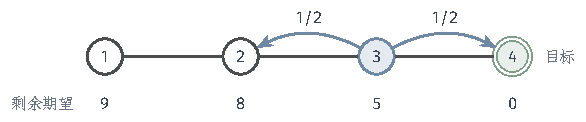
\includegraphics[width=99.24mm]{figures/03-graphs/05-matrices-and-spectra/tikz/walk-examples/hitting-path-target.pdf}
\caption{四顶点单位权路径以$4$为目标。节点下方是以该点为起点还要走的期望步数。箭头标出从$3$出发的两个去处及其概率，双圈标出目标。}
\label{fig:graph-walk-hitting-target}
\end{BookInlineFigure}

\paragraph{两个方向的首达期望不同}

从$1$到$2$只需一步。反过来从$2$到$1$就不一样了：$2$有$1/2$的概率直接到$1$，另有$1/2$的概率先走到$3$。走到$3$之后，要先从$3$绕回$2$，然后再重新尝试。

先算从$3$到$2$的平均时间。从$3$出发，$1/2$概率一步到$2$，$1/2$概率走到$4$。走到$4$后下一步必回$3$，等于白走两步回到原处。因此
\[
h_{3,2}=\tfrac{1}{2}\cdot1+\tfrac{1}{2}(2+h_{3,2}).
\]
解得$h_{3,2}=3$。

回到从$2$到$1$的问题。$1/2$概率一步到达，$1/2$概率先到$3$（一步），再从$3$回到$2$（平均$3$步），然后重新开始，
\[
h_{2,1}=\tfrac{1}{2}\cdot1+\tfrac{1}{2}(1+3+h_{2,1}).
\]
解得$h_{2,1}=5$。虽然$\{1,2\}$是一条无向边，但从两端出发绕远的机会完全不同。

在完全图$K_n$上，只要尚未命中目标，从任何非目标顶点出发，下一步命中的概率都是$1/(n-1)$。等待步数的期望就是$n-1$。

\subsection{往返时间与有效电阻}
\label{sec:graph-walk-commute-resistance}

从$i$去$j$再从$j$回$i$，总等待时间由两段组成。前一段的期望是$h_{i,j}$。前一段结束时，棋子恰好在$j$，此后每一步仍按相同规则转移，返程的条件期望都是$h_{j,i}$。两段相加，\term{往返时间}（commute time）的期望为$h_{i,j}+h_{j,i}$。

单向首达期望不对称。为了找到一个对称的表达式，先把首达方程恢复成全图形式。

将$\bm{L}\bm{h}_{:,j}$的各分量相加。$\bm{L}$的每一列和为零，因此总和也为零。已知$i\ne j$时第$i$项等于$d_i$，所以第$j$项必须抵消其余各项之和，等于$d_j-\operatorname{vol}(V)$。用$\bm{e}_j$记第$j$项为$1$、其余为$0$的列向量，全图方程为
\begin{equation}
\bm{L}\bm{h}_{:,j}=\bm{d}-\operatorname{vol}(V)\bm{e}_j.
\label{eq:graph-walk-full-hitting}
\end{equation}

右端各分量和为零，可以用伪逆$\bm{L}^\dagger$先求一个解。$\bm{L}^\dagger\bm{e}_j$取出伪逆的第$j$列，因此
\[
\bm{x}=\bm{L}^\dagger\bm{d}-\operatorname{vol}(V)\bm{L}^\dagger\bm{e}_j.
\]
这个解的第$j$项未必为零。由$\bm{L}\bm{1}=\bm{0}$，可以统一减去$x_j$后仍满足方程，同时保证$h_{j,j}=0$。展开$h_{i,j}=x_i-x_j$，得
\begin{equation}
h_{i,j}=(\bm{L}^\dagger\bm{d})_i-(\bm{L}^\dagger\bm{d})_j
+\operatorname{vol}(V)
\bigl((\bm{L}^\dagger)_{j,j}-(\bm{L}^\dagger)_{i,j}\bigr).
\label{eq:graph-walk-hitting-pseudoinverse}
\end{equation}
第一行包含度向量的信息，记录了度分配对单向首达时间的影响。正则图上度为常向量，这一部分消失。

把去程和返程相加。交换$i,j$后，第一行的两个差值恰好符号相反，抵消为零。剩下的是总加权度乘
\[
(\bm{L}^\dagger)_{i,i}+(\bm{L}^\dagger)_{j,j}
-(\bm{L}^\dagger)_{i,j}-(\bm{L}^\dagger)_{j,i}.
\]
把差向量$\bm{e}_i-\bm{e}_j$放在$\bm{L}^\dagger$的两侧相乘，展开后恰好是这四项。这正是第~\ref{sec:graph-effective-resistance}节的有效电阻二次型。

\begin{theorem}[往返时间与有效电阻]
\label{thm:graph-walk-commute-resistance}
对正权支撑连通的有限无向图，任意两点$i,j$的往返期望为
\begin{equation}
h_{i,j}+h_{j,i}
=\operatorname{vol}(V)\,R_{i,j}.
\label{eq:graph-walk-commute-time}
\end{equation}
\end{theorem}

有效电阻衡量一对顶点间的电势响应，乘以总加权度后就给出两次首达所需的平均总步数。

在四点路径上，总加权度为$1+2+2+1=6$。相邻点$1,2$之间只有一条单位电阻边，$R_{1,2}=1$，往返期望为$6$，与$h_{1,2}+h_{2,1}=1+5$一致。两端之间串联三条边，$R_{1,4}=3$，往返期望为$18$，即两个方向各$9$步。

在$n$点单位权环上，若两点沿环相隔$k$条边，两段弧的电阻分别为$k$和$n-k$，并联后得到$R=k(n-k)/n$。总度为$2n$，往返期望为$2k(n-k)$。

若把所有电导同时乘$c>0$，每步用边权除以度，转移矩阵保持不变。电阻缩小为原来的$1/c$，总加权度增为$c$倍，二者相乘后仍不变。
